%%%%%%%%%%%%%%%%%%%%%%%%%%%%%%%%%%%%%%%%%%%%%%%%%%%%%%%%%%%%%%%%%%%%%%%%%%%%%%%
%                                                                             %
% Copyright (C) 2006,2008,2012-2014 Edward d'Auvergne                         %
%                                                                             %
% This file is part of the program relax (http://www.nmr-relax.com).          %
%                                                                             %
% This program is free software: you can redistribute it and/or modify        %
% it under the terms of the GNU General Public License as published by        %
% the Free Software Foundation, either version 3 of the License, or           %
% (at your option) any later version.                                         %
%                                                                             %
% This program is distributed in the hope that it will be useful,             %
% but WITHOUT ANY WARRANTY; without even the implied warranty of              %
% MERCHANTABILITY or FITNESS FOR A PARTICULAR PURPOSE.  See the               %
% GNU General Public License for more details.                                %
%                                                                             %
% You should have received a copy of the GNU General Public License           %
% along with this program.  If not, see <http://www.gnu.org/licenses/>.       %
%                                                                             %
%%%%%%%%%%%%%%%%%%%%%%%%%%%%%%%%%%%%%%%%%%%%%%%%%%%%%%%%%%%%%%%%%%%%%%%%%%%%%%%


% Relaxation curve-fitting.
%%%%%%%%%%%%%%%%%%%%%%%%%%%

\chapter[Relaxation curve-fitting]{The $\Rone$ and $\Rtwo$ relaxation rates -- relaxation curve-fitting} \label{ch: relax-fit}
\index{relaxation curve-fitting|textbf}


\begin{figure*}[h]
  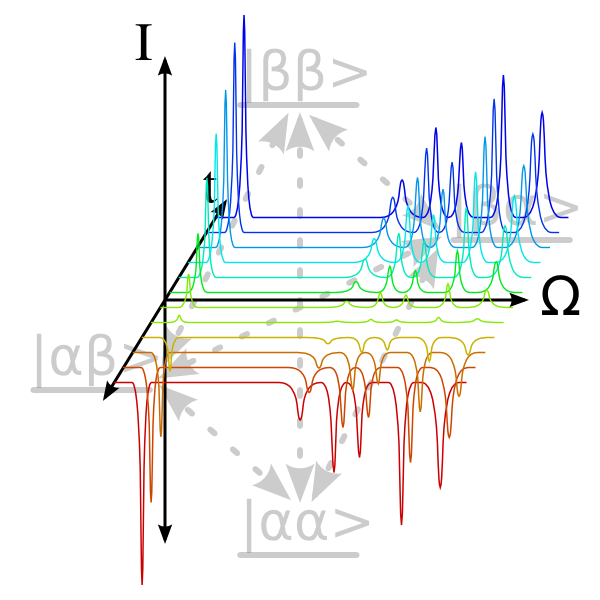
\includegraphics[width=5cm, bb=0 0 1701 1701]{graphics/analyses/r1_600x600} \hfill 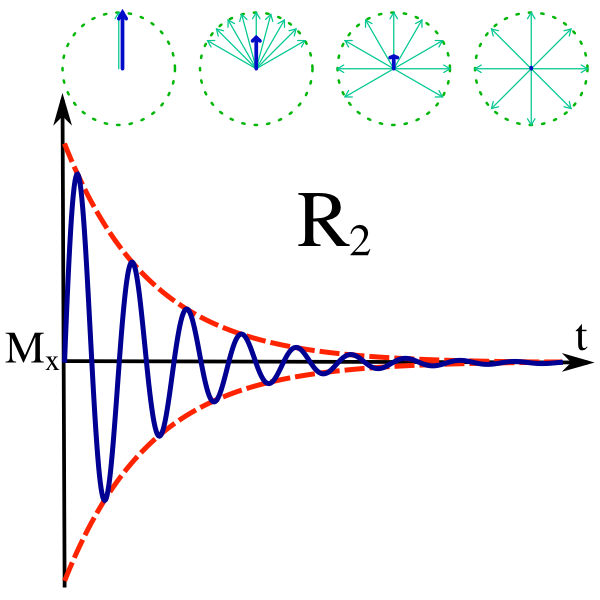
\includegraphics[width=5cm, bb=0 0 1701 1701]{graphics/analyses/r2_600x600}
\end{figure*}


% Introduction.
%%%%%%%%%%%%%%%

\section{Introduction to relaxation curve-fitting}

The fitting of exponentials to relaxation curves (relaxation curve-fitting or as used throughout this chapter abbreviated simply as relax-fit) involves a number of steps including the loading of data, the calculation of both the average peak intensity\index{peak!intensity} across replicated spectra and the standard deviations\index{standard deviation} of those peak intensities, selection of the experiment type, optimisation of the parameters of the exponential curves during the fit for each observed spin, Monte Carlo simulations\index{Monte Carlo simulation} to find the parameter errors, and saving and viewing the results.
To simplify the process a sample script will be followed step by step as was done with the NOE calculation.



% The models.
%%%%%%%%%%%%%

\section{The exponential curve models}
\label{sect: exponential curve models}

A number of different models are supported in this analysis.
These include the two parameter exponential decay to zero, the inversion recovery experiment, and the saturation recovery experiment.
These can be selected using the \uf{relax\ufus{}fit\ufsep{}select\ufus{}model} user function.

The default is the two parameter exponential decay whereby the magnetisation starts at $I_0$ and decays to zero.
It has the parameters \{$\mathrm{R}_x$, $I_0$\}.
The formula of this function is
\begin{equation}
  I(t) = I_0 e^{-\mathrm{R}_x \cdot t} ,
\end{equation}

\noindent where $I(t)$ is the peak intensity at any time point $t$, $I_0$ is the initial intensity, and $\mathrm{R}_x$ is the relaxation rate (either the $\Rone$ or $\Rtwo$).

In the inversion recovery experiment, the magnetisation starts at a negative value at $-I_0$ and relaxes to a positive $I_{\infty}$ value.
This curve consists of three parameters \{$\mathrm{R}_x$, $I_0$, $I_{\infty}$\}.
The formula is
\begin{equation}
  I(t) = I_{\infty} - I_0 e^{-\mathrm{R}_x \cdot t} .
\end{equation}

In the saturation recovery experiment, the magnetisation starts at zero and relaxes to a positive $I_{\infty}$ value.
The model consists of the two parameters \{$\mathrm{R}_x$, $I_{\infty}$\} and has the formula
\begin{equation}
  I(t) = I_{\infty} \left( 1 - e^{-\mathrm{R}_x \cdot t} \right) .
\end{equation}



% From spectra to peak intensities.
%%%%%%%%%%%%%%%%%%%%%%%%%%%%%%%%%%%

\section{From spectra to peak intensities for the relaxation rates} \label{sect: spectra to intensities}

The following subsections simply contain advice on how to go from the recorded FIDs to the peak lists ready to be input into relax.
This need not be followed -- it is simply a set of recommendations for obtaining the highest quality relaxation rates.


% Temperature control and calibration.
%~~~~~~~~~~~~~~~~~~~~~~~~~~~~~~~~~~~~~

\subsection{Temperature control and calibration} \label{sect: temperature control and calibration}


\includegraphics[bb=0 0 18 18]{graphics/oxygen_icons/128x128/status/weather-clear}

Before starting with the spectral processing, it should be noted that proper temperature control and calibration are essential for relaxation data.
Small temperature changes can have an effect on the viscosity and hence global tumbling of the molecule being studied and, as the molecular diffusion tensor is the major contributor to relaxation, any non-consistent data will likely lead to artificial motions appearing in subsequent model-free analyses.

Per-experiment temperature calibration is essential and the technique used will need to be specified for BMRB data deposition.
Note that the standard MeOH/ethylene glycol calibration of a spectrometer is of no use when you are running experiments which pump in large amounts of power into the probe head.
Although the R1 experiment should be about the same temperature as a HSQC and hence be close to the standard MeOH/ethylene glycol spectrometer calibration, the R2 CPMG or spin lock and, to a lesser extent, the NOE pre-saturation pump a lot more power into the probe head.
The power differences can either cause the temperature in the sample to be too high or too low.
This is unpredictable as the thermometer used by the VT unit is next to the coils in the probe head and not inside the NMR sample.
So the VT unit tries to control the temperature inside the probe head rather than in the NMR sample.
However between the thermometer and the sample is the water of the sample, the glass of the NMR tube, the air gap where the VT unit controls air flow and the outside components of the probe head protecting the electronics.
If the sample, the probe head or the VT unit is changed, this will have a different affect on the per-experiment temperature.
The VT unit responds differently under different conditions and may sometimes over or under compensate by a couple of degrees.
Therefore each relaxation data set from each spectrometer requires a per-experiment calibration.

Explicit temperature control techniques are also essential for relaxation data collection.
Again the technique used will be asked for by relax for BMRB data deposition.
A number of factors can cause significant temperature fluctuations between individual relaxation experiments.
This includes the daily temperature cycle of the room housing the spectrometer, different amounts of power for the individual experiments, etc.
The best methods for eliminating such problems are single scan interleaving and temperature compensation block.
Single scan interleaving is the most powerful technique for averaging the temperature fluctuations not only across different experiments, but also across the entire measurement time.
The application of off-resonance temperature compensation blocks at the start of the experiment is useful for the R2 and will normalise the temperature between the individual experiments, but single scan or single fid interleaving is nevertheless required for normalising the temperature across the entire measurement.


% Spectral processing.
%~~~~~~~~~~~~~~~~~~~~~

\subsection{Spectral processing}

For the best measurement of peak heights across the myriad of NMR spectral analysis software, it is recommend to zero fill a lot -- 8k to 16k would give the best results.
This does not increase the information content of the spectrum or decrease the errors, it simply interpolates.
Even if the NMR spectral software performs 3-point quadratic interpolation between the highest points to determine the peak height, the additional free interpolation will make the estimation more accurate.

Additionally, care must be taken to properly scale the first point as this can cause a baseline roll which will affect peak heights.
A very useful description comes directly from the \href{http://spin.niddk.nih.gov/NMRPipe/doc1/}{NMRPipe manual}:

\begin{quotation}
Depending on the delay, the first point of the FID should be adjusted before Fourier Transform.  The first point scaling factor is selected by the window function argument \prompt{-c}.

If the required first order phase P1 for the given dimension is 0.0, the first point scaling factor should be 0.5.  This is because the discrete Fourier transform does the equivalent of counting the point at t=0 twice.  If the first point is not scaled properly in this case, ridge-line baseline offsets in the spectrum will result.

In all other cases (P1 is not zero), this scale factor should be 1.0. This is because the first point of the FID no longer corresponds to t=0, and so it shouldn't be scaled. If the scale factor is not set correctly, it will introduce a baseline distortion which is either zero-order or sinusoidal, depending on what first-order phase is required. When possible, it is best to set up experiments with either exactly 0, 1/2, or 1-point delay.  There are several reasons:
\begin{itemize}
  \item Phase correction values can be determined easily.
  \item If the delay is not a multiple of 1/2 point, the phase of folded peaks will be distorted.
  \item The Hilbert transform (HT) is used, sometimes automatically, to reconstruct previously deleted imaginary data for interactive rephasing or inverse processing. But, the HT can only reconstruct imaginary data perfectly if the phase is a multiple of 1/2 point.
  \item Data with P1 = 360 have the first point t=0 missing (i.e.\ 1 point delay). Since the first point of the FID corresponds to the sum of points in the corresponding spectrum, this missing first point can be ``restored'' by adding a constant to the phased spectrum.  This can be done conveniently by automated zero-order baseline correction, as shown in table~\ref{table: NMRPipe -c}.
  
    \begin{table}
    \begin{center}
    \caption{Summary, First Point Scaling and Phase Correction}
    \begin{tabular}{llll}
    \toprule
    Delay & P1 & FID & Spectrum\\
    \midrule
    0   point &   0 & Scale -c 0.5 \\
    1/2 point & 180 & Scale -c 1.0 & Folded peaks have opposite sign \\
    1   point & 360 & Scale -c 1.0 & Use ``POLY -auto -ord 0'' \\
    \bottomrule
    \label{table: NMRPipe -c}
    \end{tabular}
    \end{center}
    \end{table}
  
\end{itemize}
\end{quotation}


Here is an example NMRPipe script designed for optimal relaxation rate extraction:
\begin{lstlisting}[language=csh]
#!/bin/csh

setenv FILEROOT $1
set PHASE=81.4

echo "\n# Fourier Transform (nmrPipe fid/*.fid to ft/*.dat)"
echo "# t2 phase is set to $PHASE"
echo "# t1 phase is set to 0.0\n"

nmrPipe -in fid/$FILEROOT.fid \
| nmrPipe -fn SOL \
| nmrPipe -fn GM -g1 15 -g2 20 -c 0.5 \
| nmrPipe -fn ZF -size 8192 \
| nmrPipe -fn FT -auto \
| nmrPipe -fn PS -p0 $PHASE -p1 0.0 -di -verb \
| nmrPipe -fn TP \
| nmrPipe -fn SP -off 0.5 -end 0.98 -pow 2 -c 0.5 \
| nmrPipe -fn ZF -size 8192 \
| nmrPipe -fn FT -auto \
| nmrPipe -fn PS -p0 0.0 -p1 0.0 -di -verb \
| nmrPipe -fn TP \
| nmrPipe -fn POLY -auto \
| nmrPipe -fn EXT -left -sw \
| nmrPipe -out ft/$FILEROOT.dat -ov
\end{lstlisting}

The script is run by suppling the FILEROOT value as a command line option so if the script is called \file{nmrpipe.sh} and the \file{var2pipe} or \file{bruk2pipe} processed file \file{R1\osus{}ncyc4.fid} is in the \directory{fid} directory, you would run:
\begin{lstlisting}[language=bash,numbers=none]
$ ./nmrpipe.sh R1_ncyc4
\end{lstlisting}

The \directory{ft} directory must exist for this script to execute.
Different experiment specific options may be needed such as:
\begin{lstlisting}[language=csh,numbers=none]
| nmrPipe -fn REV \
| nmrPipe -fn FT -neg \
| nmrPipe -fn PS -rs 2.5 \
\end{lstlisting}

The script should be changed for different phasing, first point scaling, a polynomial baseline correction added in the direct dimension or removed from the indirect dimension, solvent suppression removed or changed, and the window functions modified for optimal spectral quality.
Each system and spectrum is different, so it is recommended that to find the optimal processing that each part of the script be removed and re-added one-by-one between processing and checking of the resultant spectrum.
Note that the extraction at the end after the polynomial baseline correction in the indirect dimension is important as the baseline correction often displays a much better performance when the empty part of the spectrum is used in the calculation.



% Measuring peak intensities.
%~~~~~~~~~~~~~~~~~~~~~~~~~~~~

\subsection{Measuring peak intensities}

For the measurement of peak intensities, again care must be taken.
A read of the paper:
\begin{itemize}
  \item \bibentry{Viles01}
\end{itemize}

is highly recommended.
Despite the recommendations in the discussion of this paper, a different methodology using peak heights can be used to solve the same problems.
This will be discussed in a paper which is currently in preparation from the Gooley group.
The steps involved are:
\begin{itemize}
  \item For the first spectrum in the time series, shift the peak list to the tops of the peaks (for example using \gui{pc} in Sparky on subsets of peaks).
  \item Copy this \nth{1} spectrum list onto all spectra, shifting the peaks to the top as in the previous step.
  \item When the peak disappears into the noise, leave it at its current position and do not type \gui{pc} or equivalent.
    This will add weight to the first point in the subsequent step.
  \item Once all spectra are shifted, calculate an average peak list.
  \item Copy this average peak list onto fresh copies of all spectra.
  \item Measure peak heights using this averaged peak list.
\end{itemize}

This will produce the most accurate peak intensity measurements until better, more robust peak shape integration comes along.
This is a special technique which is designed to minimise the white-noise bias talked about in the \citet{Viles01} paper.
As the noise often decreases with the decrease in total spectral power, using the tops of the peaks means that you are actually measuring the real peak height plus positive noise in all cases.
This non-constant additional positive noise contribution can result in a double exponential in the measured data.
The technique above eliminates this as you then measure close to real peak height with the addition of white noise centred at zero -- it is both negative and positive to equal amounts -- rather than the peak high with noise contribution strongly biased towards the positive.
Where the peaks disappear, you then are measuring the pure baseplane noise.
This is fine as these white-noise data points centred at zero will help in the subsequent exponential fit in relax.

If using Sparky then, to be sure that the peak heights are properly updated, for each spectrum type \gui{pa} to select all peaks, \gui{ph} to update all selected peak heights, \gui{lt} to show the spectrum peaks window, make sure \gui{data height} is selected in the options, and then save the peak list.



% Script UI.
%%%%%%%%%%%%
\section{Relaxation curve-fitting in the prompt/script UI mode}


% The sample script.
%~~~~~~~~~~~~~~~~~~~

\subsection{Relax-fit script mode -- the sample script}

The following is a verbatim copy of the contents of the \file{sample\osus{}scripts\ossep{}relax\osus{}fit.py} file.
If your copy of the sample script is different than that below, please send an email to the relax-devel mailing list\index{mailing list!relax-devel} to tell the relax developers that the manual is out of date (see section~\ref{sect: relax-devel mailing list} on page~\pageref{sect: relax-devel mailing list}).
You will need to first copy this script to a dedicated analysis directory containing peak lists, a PDB file and a file listing unresolved spin systems, and then modify its contents to suit your specific analysis.
The script contents are:

\begin{lstlisting}
# Script for relaxation curve-fitting.

# Create the 'rx' data pipe.
pipe.create('rx', 'relax_fit')

# Load the backbone amide 15N spins from a PDB file.
structure.read_pdb('Ap4Aase_new_3.pdb')
structure.load_spins(spin_id='@N')
structure.load_spins(spin_id='@NE1')

# Spectrum names.
names = [
    'T2_ncyc1_ave',
    'T2_ncyc1b_ave',
    'T2_ncyc2_ave',
    'T2_ncyc4_ave',
    'T2_ncyc4b_ave',
    'T2_ncyc6_ave',
    'T2_ncyc9_ave',
    'T2_ncyc9b_ave',
    'T2_ncyc11_ave',
    'T2_ncyc11b_ave'
]

# Relaxation times (in seconds).
times = [
    0.0176,
    0.0176,
    0.0352,
    0.0704,
    0.0704,
    0.1056,
    0.1584,
    0.1584,
    0.1936,
    0.1936
]

# Loop over the spectra.
for i in range(len(names)):
    # Load the peak intensities.
    spectrum.read_intensities(file=names[i]+'.list', dir=data_path, spectrum_id=names[i], int_method='height')

    # Set the relaxation times.
    relax_fit.relax_time(time=times[i], spectrum_id=names[i])

# Specify the duplicated spectra.
spectrum.replicated(spectrum_ids=['T2_ncyc1_ave', 'T2_ncyc1b_ave'])
spectrum.replicated(spectrum_ids=['T2_ncyc4_ave', 'T2_ncyc4b_ave'])
spectrum.replicated(spectrum_ids=['T2_ncyc9_ave', 'T2_ncyc9b_ave'])
spectrum.replicated(spectrum_ids=['T2_ncyc11_ave', 'T2_ncyc11b_ave'])

# Peak intensity error analysis.
spectrum.error_analysis()

# Deselect unresolved spins.
deselect.read(file='unresolved', mol_name_col=1, res_num_col=2, res_name_col=3, spin_num_col=4, spin_name_col=5)

# Set the relaxation curve type.
relax_fit.select_model('exp')

# Grid search.
minimise.grid_search(inc=11)

# Minimise.
minimise.execute('newton', constraints=False)

# Monte Carlo simulations.
monte_carlo.setup(number=500)
monte_carlo.create_data()
monte_carlo.initial_values()
minimise.execute('newton', constraints=False)
monte_carlo.error_analysis()

# Save the relaxation rates.
value.write(param='rx', file='rx.out', force=True)

# Save the results.
results.write(file='results', force=True)

# Create Grace plots of the data.
grace.write(y_data_type='chi2', file='chi2.agr', force=True)    # Minimised chi-squared value.
grace.write(y_data_type='i0', file='i0.agr', force=True)    # Initial peak intensity.
grace.write(y_data_type='rx', file='rx.agr', force=True)    # Relaxation rate.
grace.write(x_data_type='relax_times', y_data_type='peak_intensity', file='intensities.agr', force=True)    # Average peak intensities.
grace.write(x_data_type='relax_times', y_data_type='peak_intensity', norm=True, file='intensities_norm.agr', force=True)    # Average peak intensities (normalised).

# Display the Grace plots.
grace.view(file='chi2.agr')
grace.view(file='i0.agr')
grace.view(file='rx.agr')
grace.view(file='intensities.agr')
grace.view(file='intensities_norm.agr')

# Save the program state.
state.save('rx.save', force=True)
\end{lstlisting}

The next sections will break this script down into its logical components and explain how these parts will be interpreted by relax.
To execute this script, please see section~\ref{sect: scripting} on page~\pageref{sect: scripting} for details.


% Initialisation of the data pipe.
%~~~~~~~~~~~~~~~~~~~~~~~~~~~~~~~~~

\subsection{Relax-fit script mode -- initialisation of the data pipe} \label{Rx initialisation}

The data pipe is simply created by the command

\begin{lstlisting}[firstnumber=3]
# Create the 'rx' data pipe.
pipe.create('rx', 'relax_fit')
\end{lstlisting}

This user function will then create a relaxation exponential curve-fitting specific data pipe labelled \promptstring{rx}.
The second argument sets the pipe type to that of the relaxation curve-fitting.
Setting the pipe type is important so that the program knows which user functions are compatible with the data pipe, for example in the steady-state NOE analysis the function \uf{minimise.execute} (see page~\pageref{uf: minimise.execute}) is meaningless as the NOE values are calculated directly rather than optimised.


% Spin systems.
%~~~~~~~~~~~~~~

\subsection{Relax-fit script mode -- setting up the spin systems}

The first thing which needs to be completed prior to any spin specific command is to generate the molecule, residue and spin data structures for storing the spin specific data.
In the sample script above this is generated from a PDB file, however a plain text file with the sequence information can be used instead (see the \uf{sequence\ufsep{}read} user function on page~\pageref{uf: sequence.read} for more details).
In the case of the sample script, the command

\begin{lstlisting}[firstnumber=6]
# Load the backbone amide 15N spins from a PDB file.
structure.read_pdb(name, 'Ap4Aase_new_3.pdb')
\end{lstlisting}
\index{PDB}

will load the PDB file \file{Ap4Aase\osus{}new\osus{}3.pdb} into relax.
Then 

\begin{lstlisting}[firstnumber=8]
structure.load_spins(spin_id='@N')
structure.load_spins(spin_id='@NE1')
\end{lstlisting}

will generate the molecule, residue, and spin sequence for the current data pipe.
In this situation there will be a single spin system per residue generated corresponding to the backbone amide nitrogens as well as $^{15}$N spins set up for the tryptophan indole nitrogens.
Although the 3D coordinates have been loaded into the program from the PDB file, this structural information serves no purpose when calculating $\Rone$ and $\Rtwo$ values.


% Loading the data.
%~~~~~~~~~~~~~~~~~~

\subsection{Relax-fit script mode -- loading the data} \label{sect: Rx data loading}

To load the peak intensities\index{peak!intensity} into relax the \uf{spectrum\ufsep{}read\ufus{}intensities} and \uf{relax\ufus{}fit\ufsep{}relax\ufus{}times} user functions are executed.
Important keyword arguments for these user functions are the file name and directory, the spectrum identification string and the relaxation time period of the experiment in seconds.
By default the file format will be automatically detected.
Currently Sparky\index{software!Sparky}, XEasy\index{software!XEasy}, NMRView\index{software!NMRView}, and generic columnar formatted peak lists are supported.
To be able to import any other type of format please send an email to the relax development mailing list\index{mailing list!relax-devel} with the details of the format.
Adding support for new formats is trivial.
The following series of commands -- an expansion of the \prompt{for} loop in the sample script -- will load peak intensities from six different relaxation periods, four of which have been duplicated, from Sparky peak lists with the peak heights in the 10$^{\textrm{th}}$ column.

\begin{lstlisting}[numbers=none]
spectrum.read_intensities('T2_ncyc1.list',   spectrum_id='1', int_col=10)
relax_fit.relax_time(spectrum_id='1',   time=0.0176)
spectrum.read_intensities('T2_ncyc1b.list',  spectrum_id='1b', int_col=10)
relax_fit.relax_time(spectrum_id='1b',  time=0.0176)
spectrum.read_intensities('T2_ncyc2.list',   spectrum_id='2', int_col=10)
relax_fit.relax_time(spectrum_id='2',   time=0.0352)
spectrum.read_intensities('T2_ncyc4.list',   spectrum_id='4', int_col=10)
relax_fit.relax_time(spectrum_id='4',   time=0.0704)
spectrum.read_intensities('T2_ncyc4b.list',  spectrum_id='4b', int_col=10)
relax_fit.relax_time(spectrum_id='4b',  time=0.0704)
spectrum.read_intensities('T2_ncyc6.list',   spectrum_id='6', int_col=10)
relax_fit.relax_time(spectrum_id='6',   time=0.1056)
spectrum.read_intensities('T2_ncyc9.list',   spectrum_id='9', int_col=10)
relax_fit.relax_time(spectrum_id='9',   time=0.1584)
spectrum.read_intensities('T2_ncyc9b.list',  spectrum_id='9b', int_col=10)
relax_fit.relax_time(spectrum_id='9b',  time=0.1584)
spectrum.read_intensities('T2_ncyc11.list',  spectrum_id='11', int_col=10)
relax_fit.relax_time(spectrum_id='11',  time=0.1936)
spectrum.read_intensities('T2_ncyc11b.list', spectrum_id='11b', int_col=10)
relax_fit.relax_time(spectrum_id='11b', time=0.1936)
\end{lstlisting}

The replicated spectra a set up with the commands

\begin{lstlisting}[firstnumber=47]
# Specify the duplicated spectra.
spectrum.replicated(spectrum_ids=['T2_ncyc1_ave', 'T2_ncyc1b_ave'])
spectrum.replicated(spectrum_ids=['T2_ncyc4_ave', 'T2_ncyc4b_ave'])
spectrum.replicated(spectrum_ids=['T2_ncyc9_ave', 'T2_ncyc9b_ave'])
spectrum.replicated(spectrum_ids=['T2_ncyc11_ave', 'T2_ncyc11b_ave'])
\end{lstlisting}

Note that the relaxation time period should be calculated directly from the pulse sequence (as the sum of delays and pulses for the period), as the estimated time may not match the real time.
For the Sparky peak lists, by default relax assumes that the intensity value is in the 4$^{\textrm{th}}$ column.
A typical file looks like:

{\scriptsize \begin{verbatim}
     Assignment         w1         w2   Data Height

        LEU3N-HN    122.454      8.397       129722
        GLY4N-HN    111.999      8.719       422375
        SER5N-HN    115.085      8.176       384180
        MET6N-HN    120.934      8.812       272100
        ASP7N-HN    122.394      8.750       174970
        SER8N-HN    113.916      7.836       218762
       GLU11N-HN    122.194      8.604        30412
       GLY12N-HN    110.525      9.028        90144
\end{verbatim}}

By supplying the \keyword{int\_col} argument to the \uf{spectrum\ufsep{}read\ufus{}intensities} user function, this can be changed.
A typical XEasy file will look like:

{\scriptsize \begin{verbatim}
 No.  Color    w1      w2     ass. in w1     ass. in w2    Volume     Vol. Err.  Method  Comment

   2    2    10.014 134.221   HN  21 LEU      N  21 LEU    7.919e+03  0.00e+00     m
   3    2    10.481 132.592  HE1  79 TRP    NE1  79 TRP    1.532e+04  0.00e+00     m
  17    2     9.882 129.041   HN 110 PHE      N 110 PHE    9.962e+03  0.00e+00     m
  18    2     8.757 128.278   HN  52 ASP      N  52 ASP    2.041e+04  0.00e+00     m
  19    2    10.086 128.297   HN  69 SER      N  69 SER    9.305e+03  0.00e+00     m
  20    3     9.111 127.707   HN  15 ARG      N  15 ARG    9.714e+03  0.00e+00     m
\end{verbatim}}

where the peak height is in the \prompt{Volume} column.
And for an NMRView file:

{\tiny \begin{verbatim}
label dataset sw sf
H1 N15
cNTnC_noe0.nv
2505.63354492 1369.33557129
499.875 50.658000946
H1.L H1.P H1.W H1.B H1.E H1.J H1.U N15.L N15.P N15.W N15.B N15.E N15.J N15.U vol int stat comment flag0
0 {70.HN} 10.75274 0.02954 0.05379 ++ 0.0 {} {70.N} 116.37241 0.23155 0.35387 ++ 0.0 {} -6.88333129883 -0.1694 0 {} 0
1 {72.HN} 9.67752 0.03308 0.05448 ++ 0.0 {} {72.N} 126.41302 0.27417 0.37217 ++ 0.0 {} -5.49038267136 -0.1142 0 {} 0
2 {} 8.4532 0.02331 0.05439 ++ 0.0 {} {} 122.20137 0.38205 0.33221 ++ 0.0 {} -2.58034267191 -0.1320 0 {} 0
\end{verbatim}}


% The rest of the setup.
%~~~~~~~~~~~~~~~~~~~~~~~

\subsection{Relax-fit script mode -- the rest of the setup} \label{sect: Rx setup fin}

Once all the peak intensity data has been loaded a few calculations are required prior to optimisation.
Firstly the peak intensities for individual spins needs to be averaged across replicated spectra.
The peak intensity errors also have to be calculated using the standard deviation formula.
These two operations are executed by the user function

\begin{lstlisting}[firstnumber=53]
# Peak intensity error analysis.
spectrum.error_analysis()
\end{lstlisting}

Any spins which cannot be resolved due to peak overlap were included in a file called \file{unresolved}.
This file can consist of optional columns of the molecule name, the residue name and number, and the spin name and number.
The matching spins are excluded from the analysis by the user function

\begin{lstlisting}[firstnumber=56]
# Deselect unresolved spins.
deselect.read(file='unresolved', mol_name_col=1, res_num_col=2, res_name_col=3, spin_num_col=4, spin_name_col=5)
\end{lstlisting}

Finally the experiment type is specified by the command

\begin{lstlisting}[firstnumber=59]
# Set the relaxation curve type.
relax_fit.select_model('exp')
\end{lstlisting}

The argument \promptstring{exp} sets the relaxation curve to a two parameter \{$\mathrm{R}_x$, $I_0$\} exponential which decays to zero.
Changing the user function argument to \promptstring{inv} will select the inversion recovery experiment, and changing it to \promptstring{sat} will select the saturation recovery experiment (see section~\ref{sect: exponential curve models} on page~\pageref{sect: exponential curve models}).



% Optimisation.
%~~~~~~~~~~~~~~

\subsection{Relax-fit script mode -- optimisation of exponential curves}

Now that everything has been setup minimisation can be used to optimise the parameter values.
Firstly a grid search is applied to find a rough starting position for the subsequent optimisation algorithm.
Eleven increments per dimension of the model (in this case the two dimensions \{$\mathrm{R}_x$, $I_0$\}) is sufficient.
The user function for executing the grid search is

\begin{lstlisting}[firstnumber=62]
# Grid search.
minimise.grid_search(inc=11)
\end{lstlisting}

The next step is to select one of the minimisation algorithms to optimise the model parameters

\begin{lstlisting}[firstnumber=65]
# Minimise.
minimise.execute('newton', constraints=False)
\end{lstlisting}



% Error analysis.
%~~~~~~~~~~~~~~~~

\subsection{Relax-fit script mode -- error analysis}

Only one technique adequately estimates parameter errors when the parameter values where found by optimisation -- Monte Carlo simulations\index{Monte Carlo simulation}.
In relax this can be implemented by using a series of functions from the \uf{monte\ufus{}carlo} user function class.
Firstly the number of simulations needs to be set

\begin{lstlisting}[firstnumber=68]
# Monte Carlo simulations.
monte_carlo.setup(number=500)
\end{lstlisting}

For each simulation, randomised relaxation curves will be fit using exactly the same methodology as the original exponential curves.
These randomised curves are created by back calculation from the fitted model parameter values and then each point on the curve randomised using the error values set earlier in the script

\begin{lstlisting}[firstnumber=70]
monte_carlo.create_data()
\end{lstlisting}

As a grid search for each simulation would be too computationally expensive, the starting point for optimisation for each simulation can be set to the position of the optimised parameter values of the model

\begin{lstlisting}[firstnumber=71]
monte_carlo.initial_values()
\end{lstlisting}

Then exactly the same optimisation as was used for the model can be performed

\begin{lstlisting}[firstnumber=72]
minimise.execute('newton', constraints=False)
\end{lstlisting}

The parameter errors are then determined as the standard deviation of the optimised parameter values of the simulations

\begin{lstlisting}[firstnumber=73]
monte_carlo.error_analysis()
\end{lstlisting}


% Finishing off.
%~~~~~~~~~~~~~~~

\subsection{Relax-fit script mode -- finishing off}

To finish off, the script first saves the relaxation rates together with their errors in a simple text file

\begin{lstlisting}[firstnumber=75]
# Save the relaxation rates.
value.write(param='rx', file='rx.out', force=True)
\end{lstlisting}

Grace plots are created and viewed

\begin{lstlisting}[firstnumber=81]
# Create Grace plots of the data.
grace.write(y_data_type='chi2', file='chi2.agr', force=True)    # Minimised chi-squared value.
grace.write(y_data_type='i0', file='i0.agr', force=True)    # Initial peak intensity.
grace.write(y_data_type='rx', file='rx.agr', force=True)    # Relaxation rate.
grace.write(x_data_type='relax_times', y_data_type='peak_intensity', file='intensities.agr', force=True)    # Average peak intensities.

grace.write(x_data_type='relax_times', y_data_type='peak_intensity', norm=True, file='intensities_norm.agr', force=True)    # Average peak intensities (normalised).
\end{lstlisting}

and viewed

\begin{lstlisting}[firstnumber=88]
# Display the Grace plots.
grace.view(file='chi2.agr')
grace.view(file='i0.agr')
grace.view(file='rx.agr')
grace.view(file='intensities.agr')
grace.view(file='intensities_norm.agr')
\end{lstlisting}

and finally the program state is saved for future reference

\begin{lstlisting}[firstnumber=95]
# Save the program state.
state.save(file='rx.save', force=True)
\end{lstlisting}



% GUI.
%%%%%%

\newpage
\section{The relaxation curve-fitting auto-analysis in the GUI}

The $\Rone$ and $\Rtwo$ relaxation rates can be calculated using the relax GUI (see Figures~\ref{fig: screenshot: R1 analysis} and~\ref{fig: screenshot: R2 analysis}).
These auto-analyses can be selected using the analysis selection wizard (Figure~\ref{fig: screenshot: analysis wizard} on page~\pageref{fig: screenshot: analysis wizard}).
Just as with the steady-state NOE in the next chapter, these auto-analyses are very similar in spirit to the sample script described in this chapter, though the Grace 2D visualisation is more advanced.
If you have read this chapter, the usage of these analyses should be self explanatory.

As in the script/prompt UI section above, the example of protein $^{15}$N $\Rone$ relaxation analysis will be performed in the following sections.
To keep track of all the messages relax produces for future reference, you can run the relax GUI with the following command line arguments:

\example{\$ relax --log log --gui}

The messages will then appear both in the relax controller window (see Figure~\ref{fig: screenshot: relax controller} on page~\pageref{fig: screenshot: relax controller}) and in the \file{log} file.


% Initialisation of the data pipe.
%~~~~~~~~~~~~~~~~~~~~~~~~~~~~~~~~~

\subsection{Relax-fit GUI mode -- initialisation of the data pipe}

To begin the analysis, launch the analysis selection wizard (see Figure~\ref{fig: screenshot: analysis wizard} on page \pageref{fig: screenshot: analysis wizard}).
Select either the $\Rone$ or $\Rtwo$ analyses, and change the name of the analysis if you plan on running multiple analyses from different field strengths in one relax instance.

\begin{minipage}[h]{\linewidth}
  \centerline{
    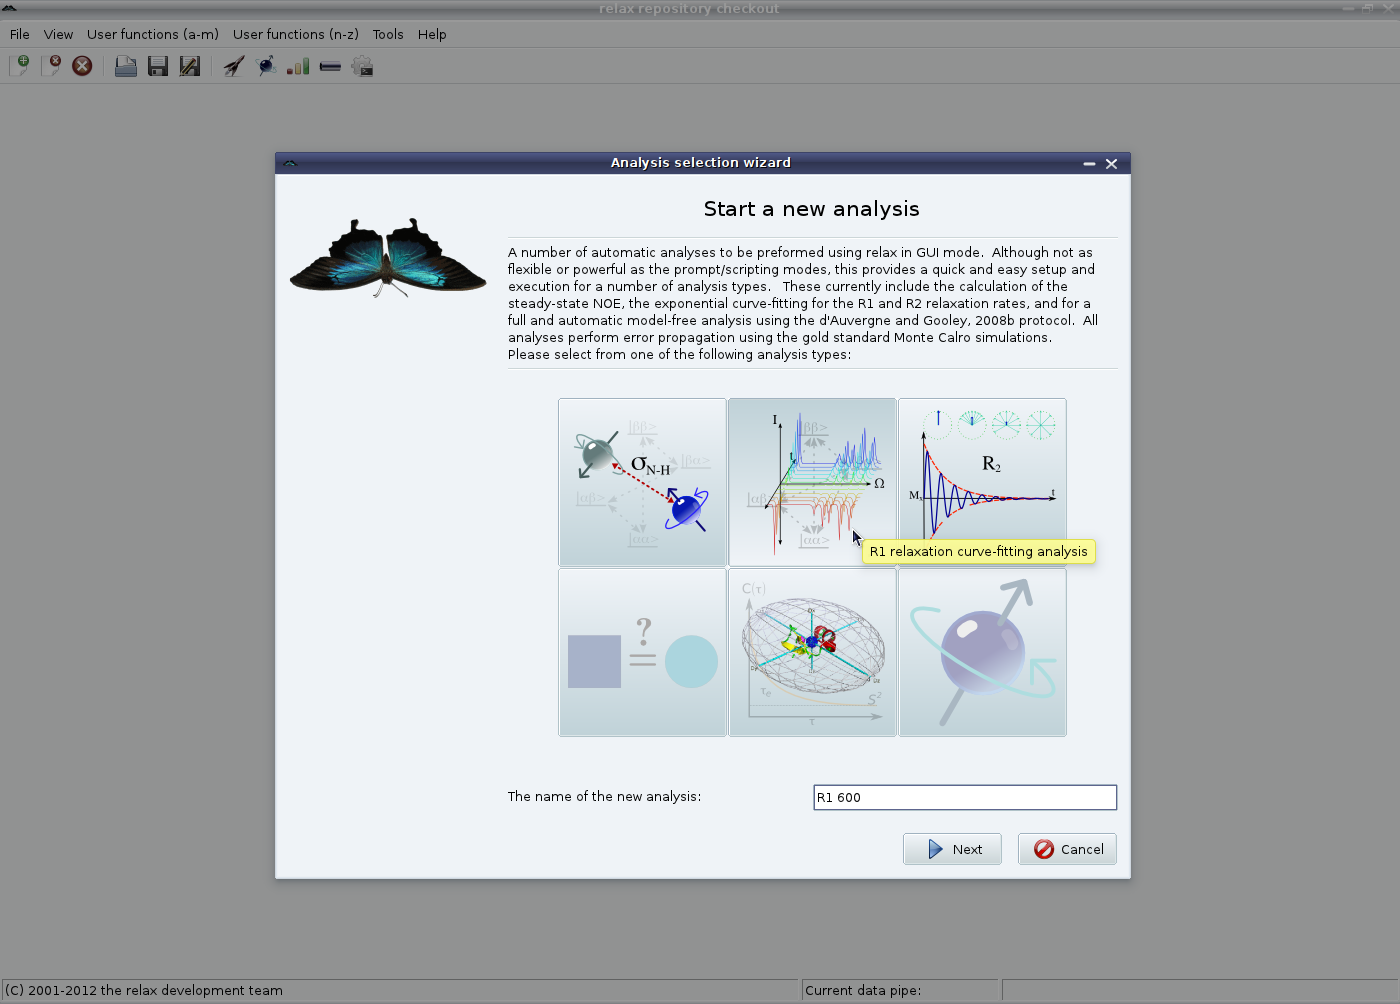
\includegraphics[
      width=0.8\textwidth,
      bb=14 14 1415 1019
    ]
    {graphics/screenshots/r1_analysis/analysis_wizard1}
  }
\end{minipage}

Then click on the \guibutton{Next} button.
On the second page click on \guibutton{Start} to commence the analysis -- this second part of the wizard does not need to be changed.
For the $\Rone$ and $\Rtwo$ analyses in the GUI, a data pipe bundle containing only a single data pipe for that analysis will be created.
This data pipe bundle can be safely ignored.

\begin{minipage}[h]{\linewidth}
  \centerline{
    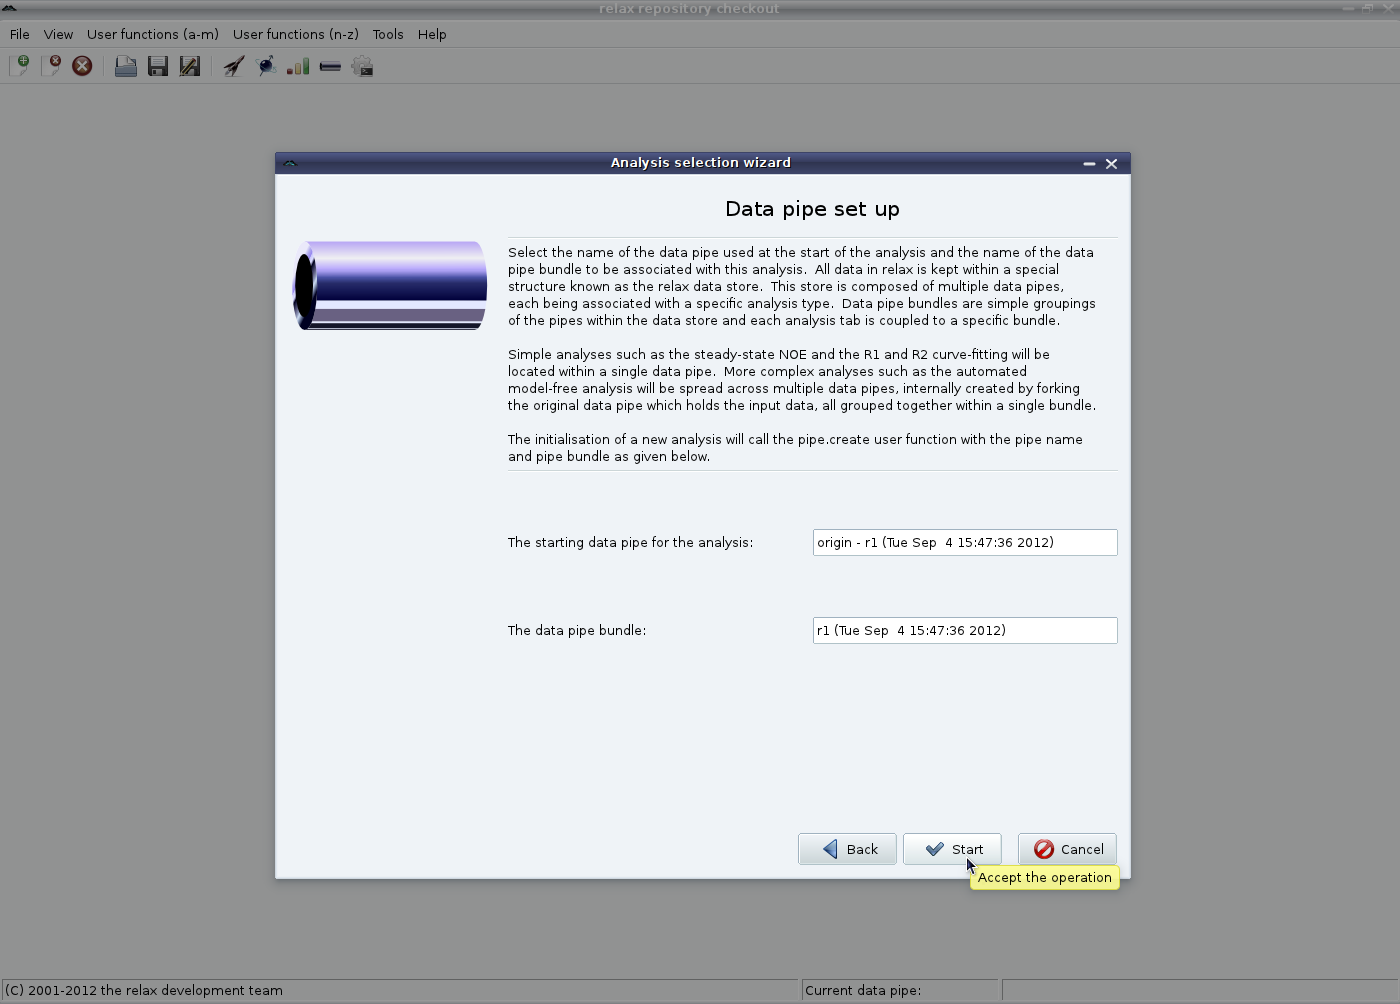
\includegraphics[
      width=0.8\textwidth,
      bb=14 14 1415 1019
    ]
    {graphics/screenshots/r1_analysis/analysis_wizard2}
  }
\end{minipage}


% General setup.
%~~~~~~~~~~~~~~~

\subsection{Relax-fit GUI mode -- general setup}

You will now be presented with a blank analysis tab:

\begin{minipage}[h]{\linewidth}
  \centerline{
    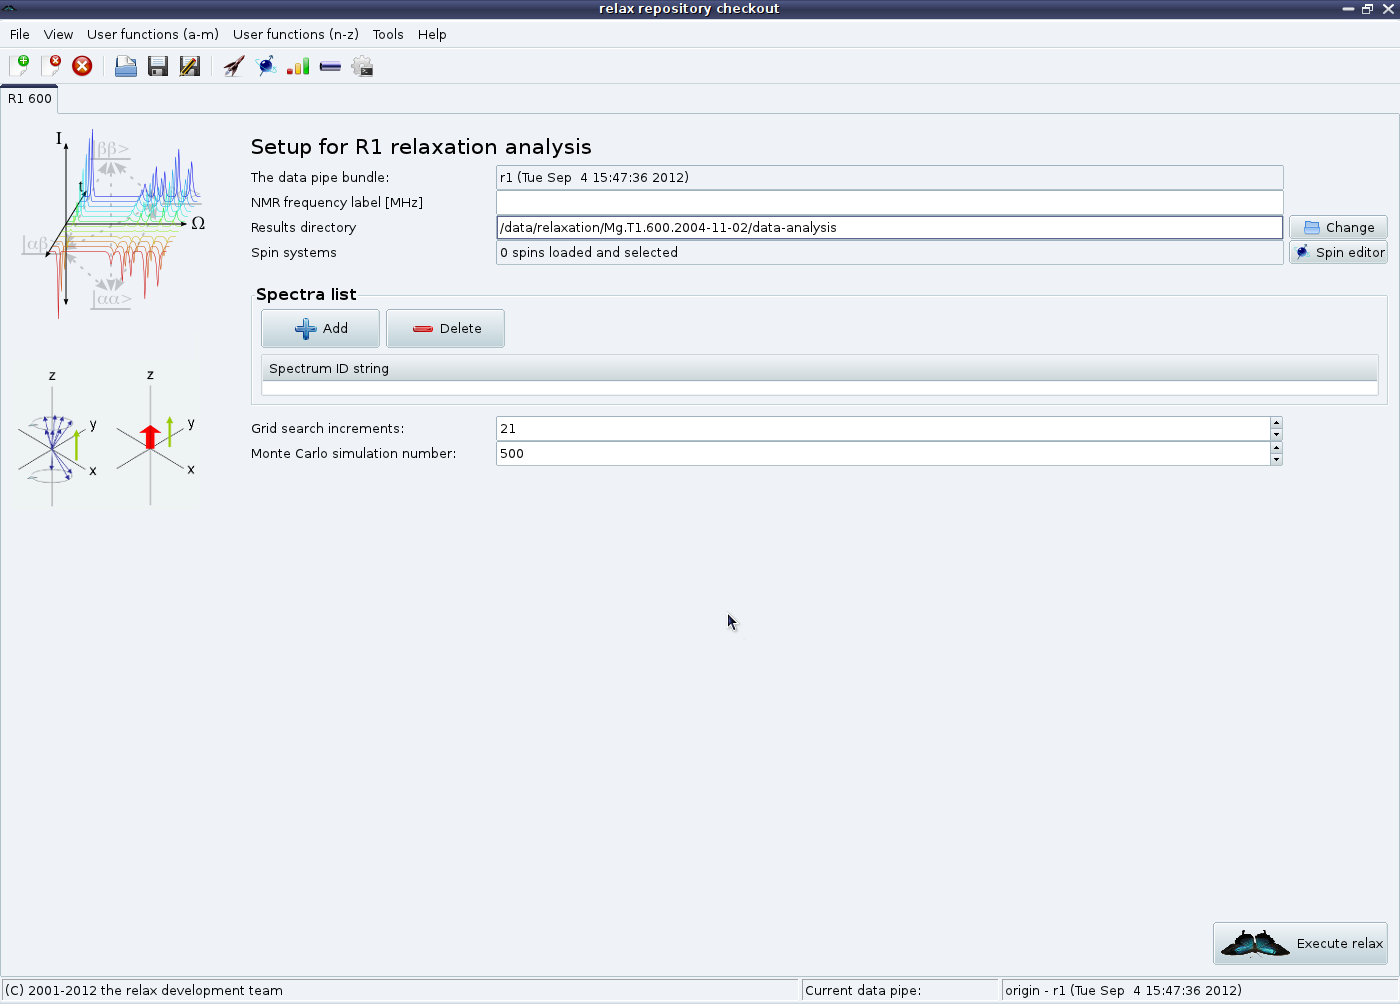
\includegraphics[
      width=0.8\textwidth,
      bb=14 14 1415 1019
    ]
    {graphics/screenshots/r1_analysis/blank}
  }
\end{minipage}

Here there are two things unique to the GUI which need to be preformed:
\begin{description}
  \item[NMR frequency label:]  First set the NMR frequency label.
    This is only used for the name of the output file.
    For example if you set the label to \guistring{1200}, the file \file{r1.1200.out} will be created at the end of the analysis.
  \item[Results directory:]  All of the automatically created results and Grace files will be placed into this directory.
    The \gui{Results directory} can now be changed.
\end{description}


% Spin systems.
%~~~~~~~~~~~~~~

\subsection{Relax-fit GUI mode -- setting up the spin systems}

As the relaxation data is at the level of the spins, the molecule, residue and spin data structures need to be set up.
In the $\Rone$ and $\Rtwo$ GUI analysis tabs, there is a special \gui{Spin systems} GUI element designed for this.
This will initially say \gui{0 spins loaded and selected}.
Click on the \guibutton{Spin editor} button to launch the spin viewer window.
The steps for setting up the spin containers using PDB files are described in section~\ref{sect: GUI - structural data} on page~\pageref{sect: GUI - structural data} or for sequence files in section~\ref{sect: GUI - sequence file} on page~\pageref{sect: GUI - sequence file}.


% Unresolved spins.
%~~~~~~~~~~~~~~~~~~

\subsection{Relax-fit GUI mode -- unresolved spins}

As in the prompt/script UI section~\ref{sect: Rx setup fin}, the spins can be deselected at this point using the same \file{unresolved} file.
This is described in detail in section~\ref{sect: GUI - deselect spins} on page~\pageref{sect: GUI - deselect spins}.



% Loading the data.
%~~~~~~~~~~~~~~~~~~

\subsection{Relax-fit GUI mode -- loading the data}

At this stage, the peak intensity data needs to be loaded.
In both the $\Rone$ and $\Rtwo$ analysis tabs is a \gui{Spectra list} GUI element.
Click on the \guibutton{Add} button to launch the peak intensity loading wizard:

\begin{minipage}[h]{\linewidth}
  \centerline{
    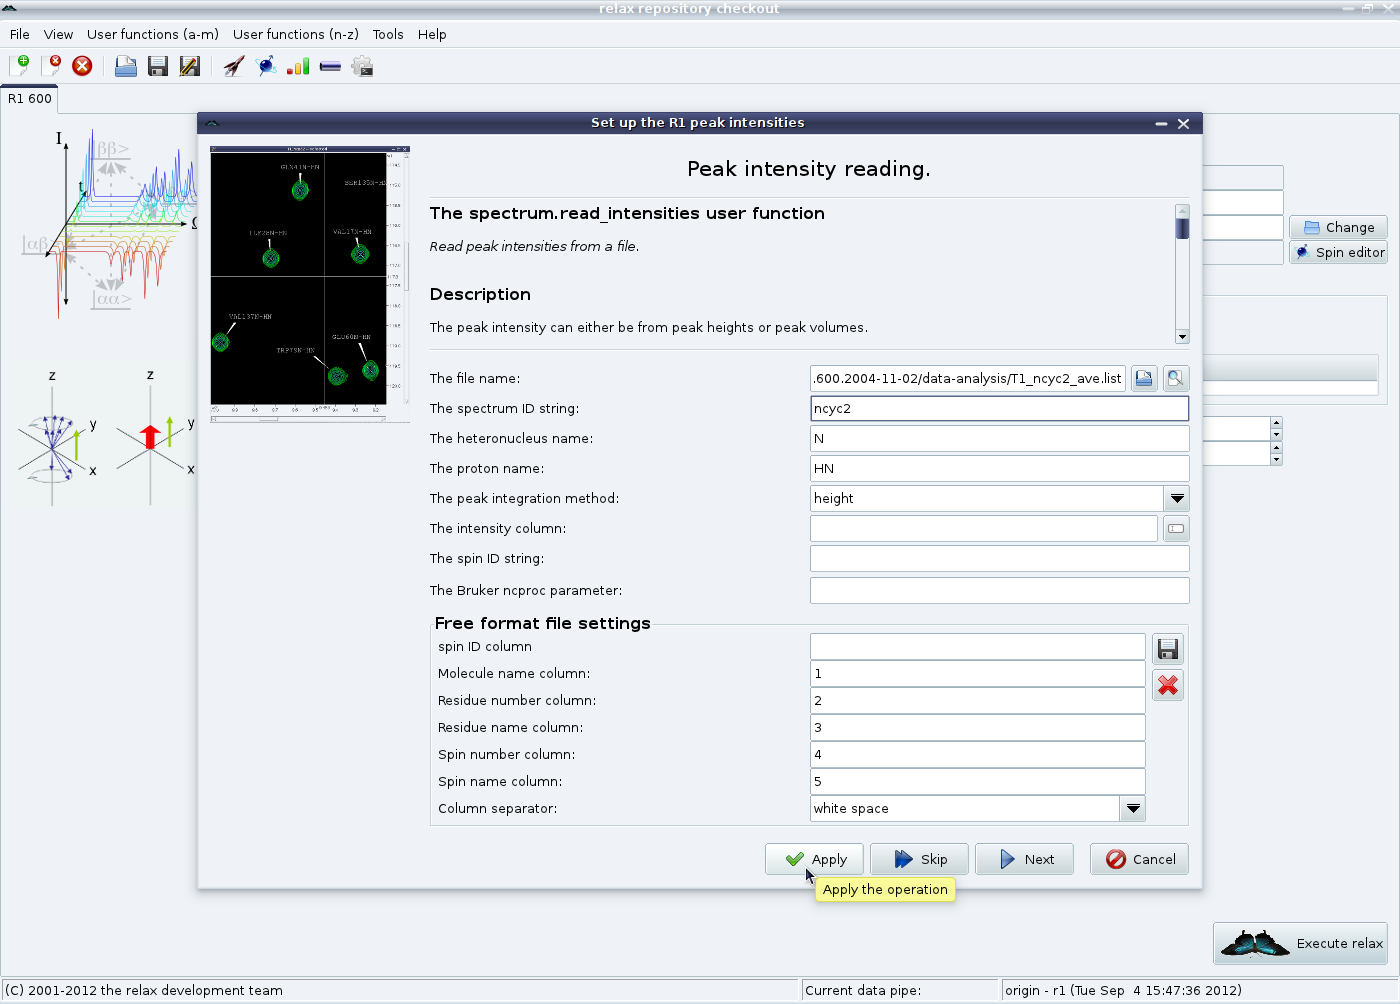
\includegraphics[
      width=0.8\textwidth,
      bb=14 14 1415 1019
    ]
    {graphics/screenshots/r1_analysis/peak_intensity_bb_peaks}
  }
\end{minipage}

In this example, a Sparky peak list containing the peak heights determined from the averaged chemical shift positions for all spectra will be loaded.
Set the spectrum ID string to a unique value.
Click on \guibutton{Next}.
This will most likely cause a \prompt{RelaxWarning} message to appear for all peak list elements which do not correspond to any spins loaded into the relax data store:

\begin{minipage}[h]{\linewidth}
  \centerline{
    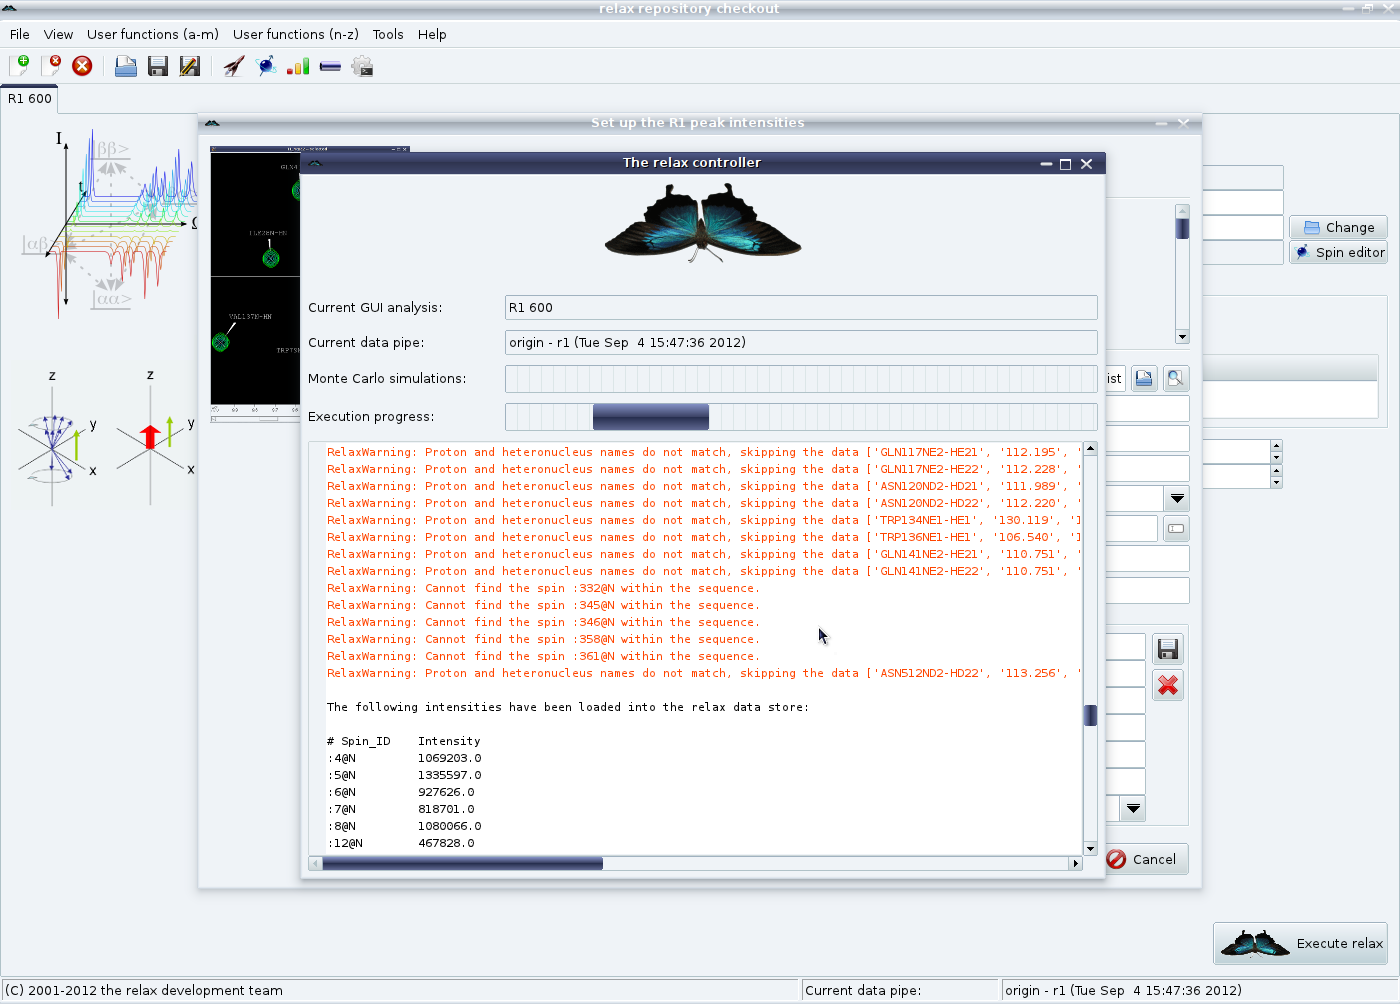
\includegraphics[
      width=0.8\textwidth,
      bb=14 14 1415 1019
    ]
    {graphics/screenshots/r1_analysis/peak_intensity_warnings}
  }
\end{minipage}

These messages must be carefully checked to be sure that the correct data has been loaded.
A \prompt{RelaxError} might be thrown if the peak list is corrupted or if the dimension has been incorrectly given.
In this case check the message, go \guibutton{Back}, fix the problem, and click on \guibutton{Next} again.
Then click on \guibutton{Next}.
You should now see the error type page:

\begin{minipage}[h]{\linewidth}
  \centerline{
    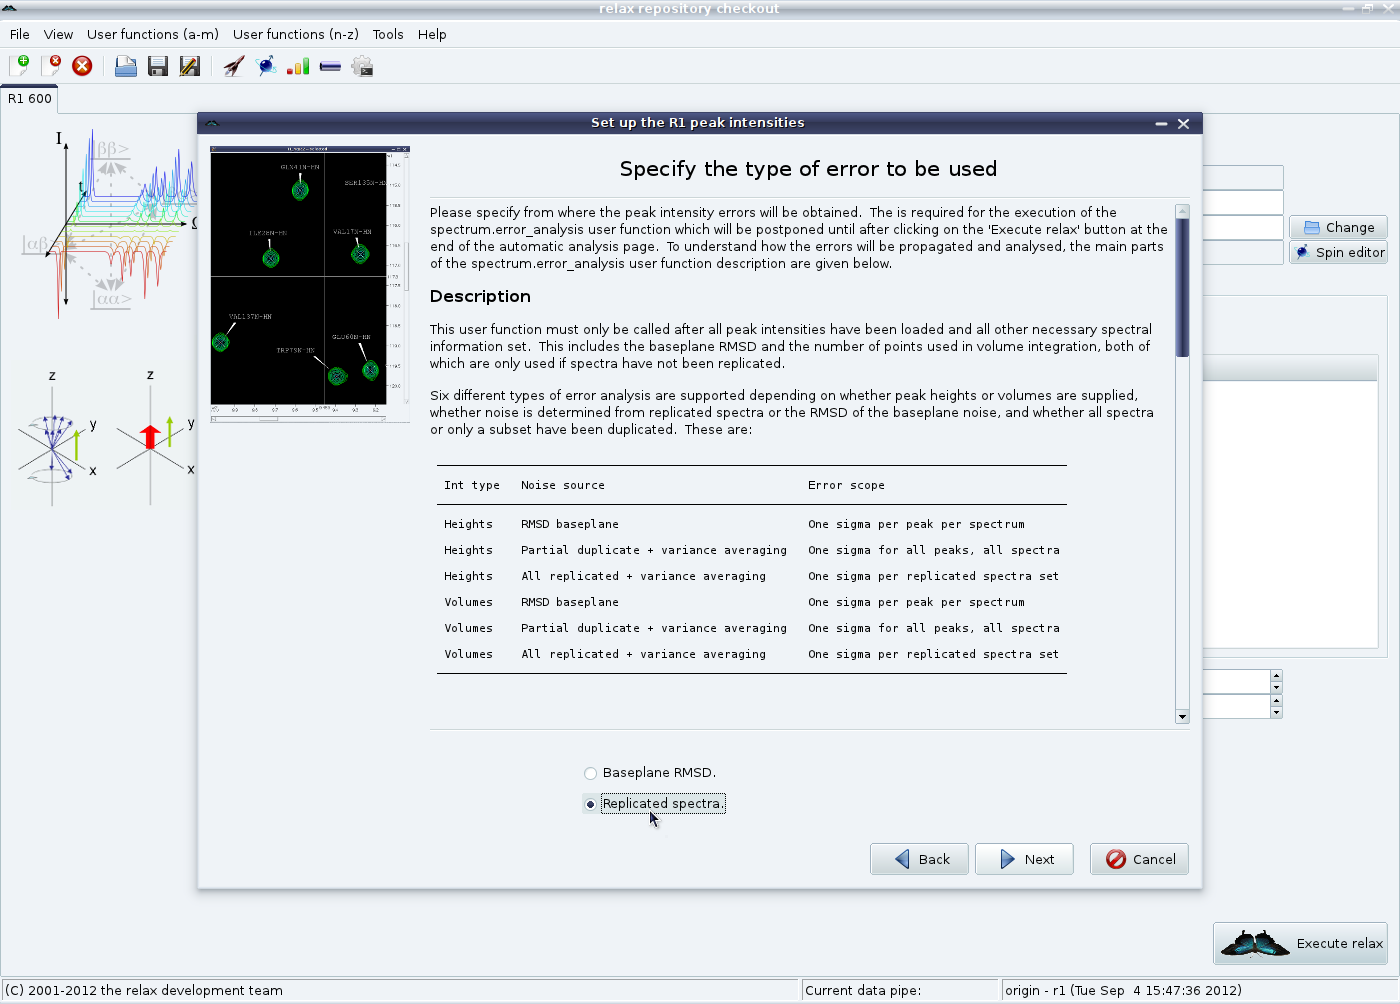
\includegraphics[
      width=0.8\textwidth,
      bb=14 14 1415 1019
    ]
    {graphics/screenshots/r1_analysis/peak_intensity_err_type}
  }
\end{minipage}

The description for this wizard page should be very carefully read -- it will tell you about all of the error analysis options available and how these are implemented in relax.
For the protein relaxation example, replicated spectra have been collected.
Therefore the option \gui{Replicated spectra} will be chosen.
The \gui{Baseplane RMSD} option is documented in the NOE chapter.
After clicking on \guibutton{Next} you will see:

\begin{minipage}[h]{\linewidth}
  \centerline{
    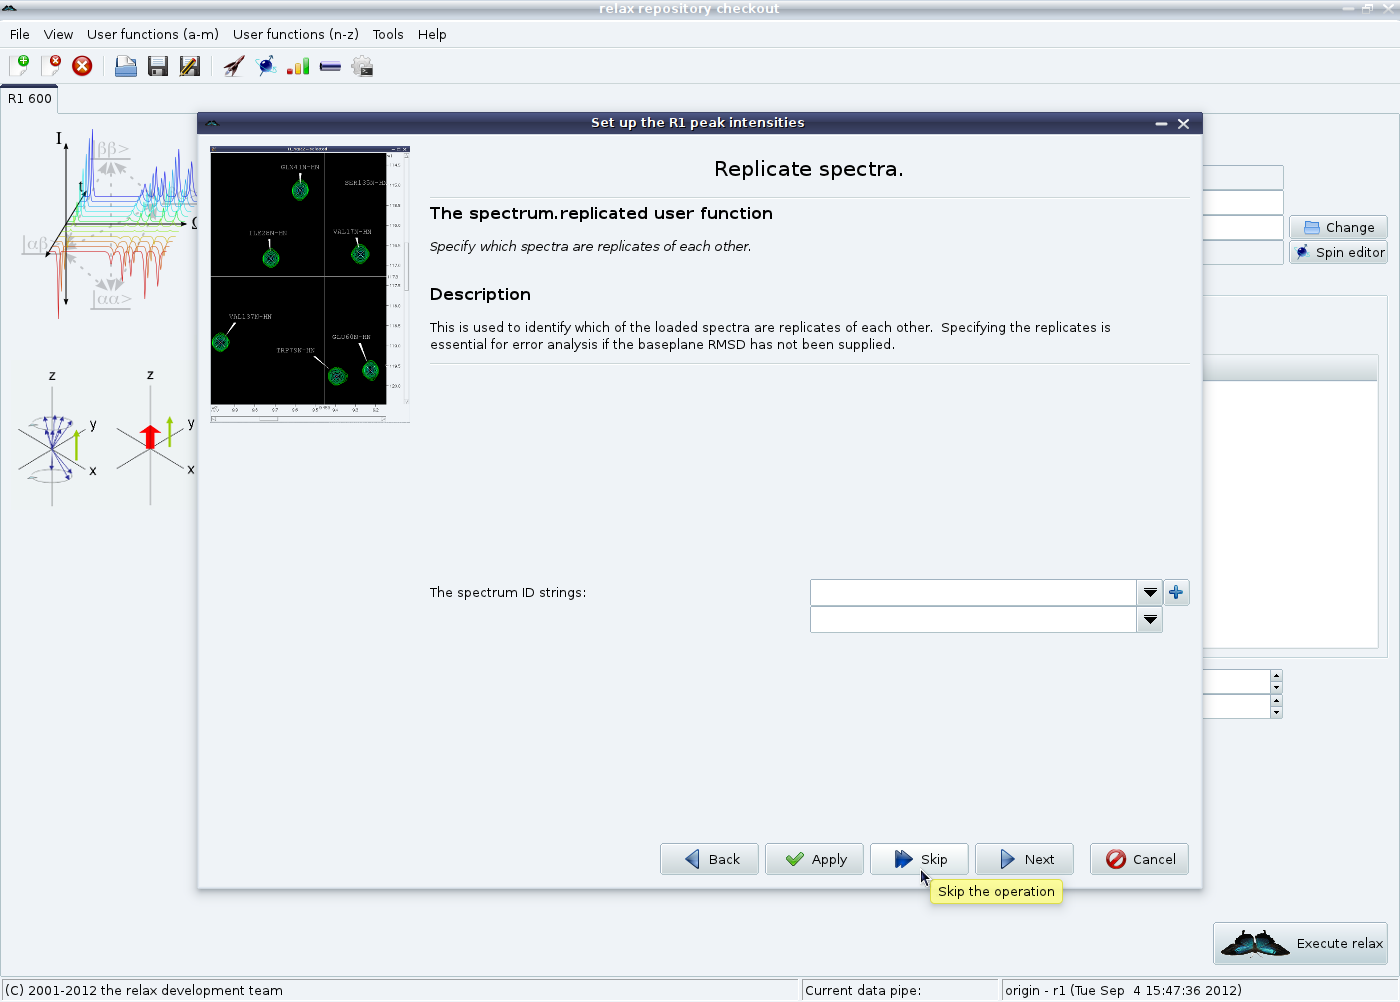
\includegraphics[
      width=0.8\textwidth,
      bb=14 14 1415 1019
    ]
    {graphics/screenshots/r1_analysis/peak_intensity_replicates1}
  }
\end{minipage}

For the first of the duplicate spectra, or any spectrum without a duplicate, you can click on the \guibutton{Skip} button.
If this is the second spectrum you have loaded from a duplicated set, select the two replicated spectra and then click on \guibutton{Next}:

\begin{minipage}[h]{\linewidth}
  \centerline{
    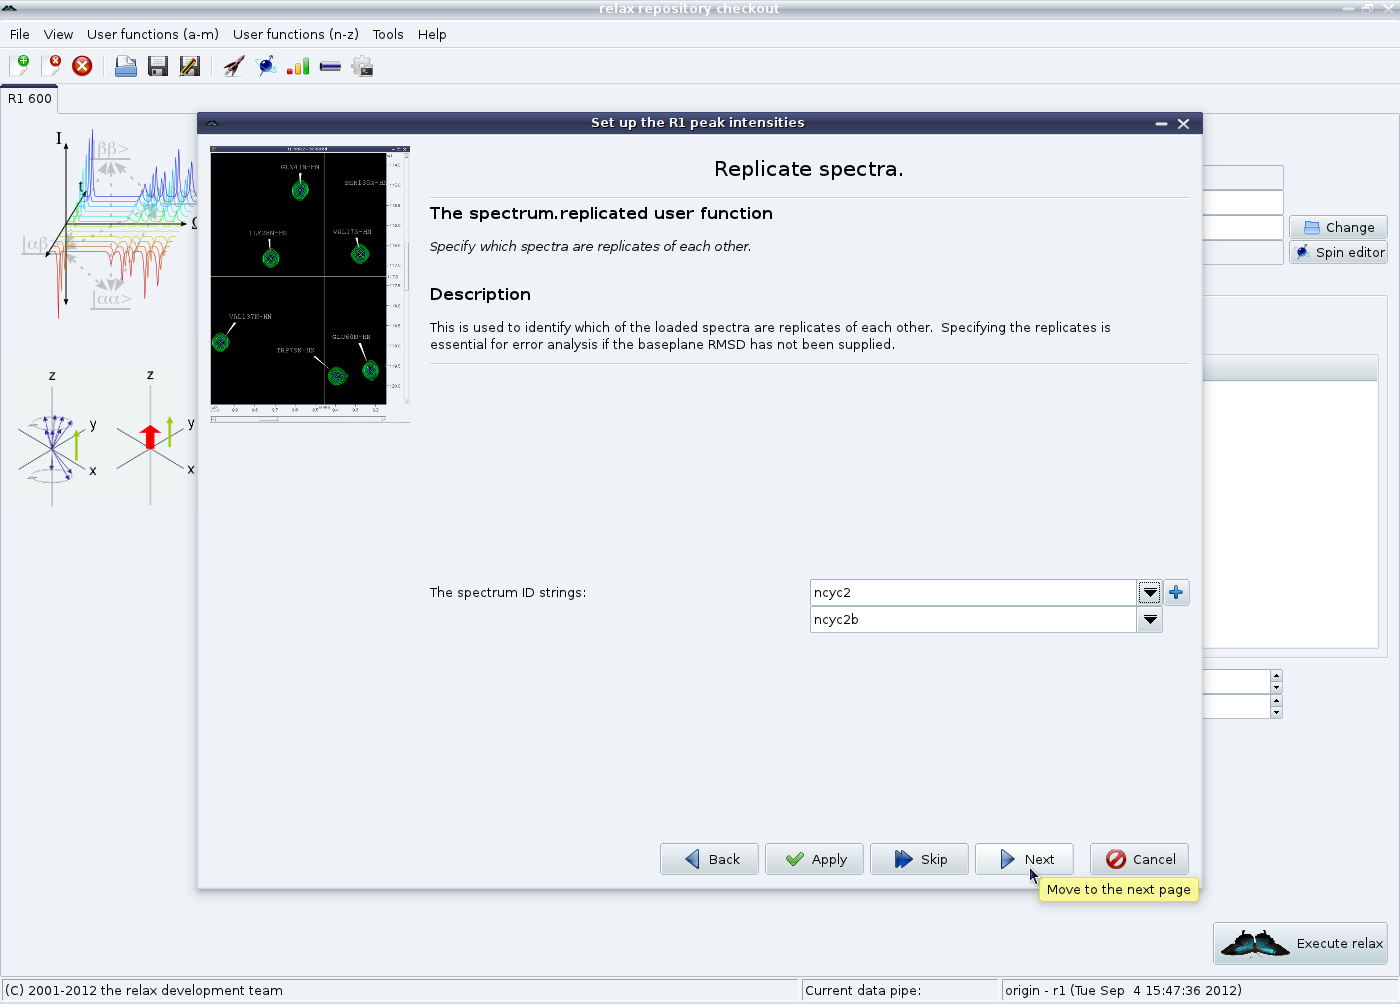
\includegraphics[
      width=0.8\textwidth,
      bb=14 14 1415 1019
    ]
    {graphics/screenshots/r1_analysis/peak_intensity_replicates2}
  }
\end{minipage}

Finally set the relaxation time period for this experiment in seconds:

\begin{minipage}[h]{\linewidth}
  \centerline{
    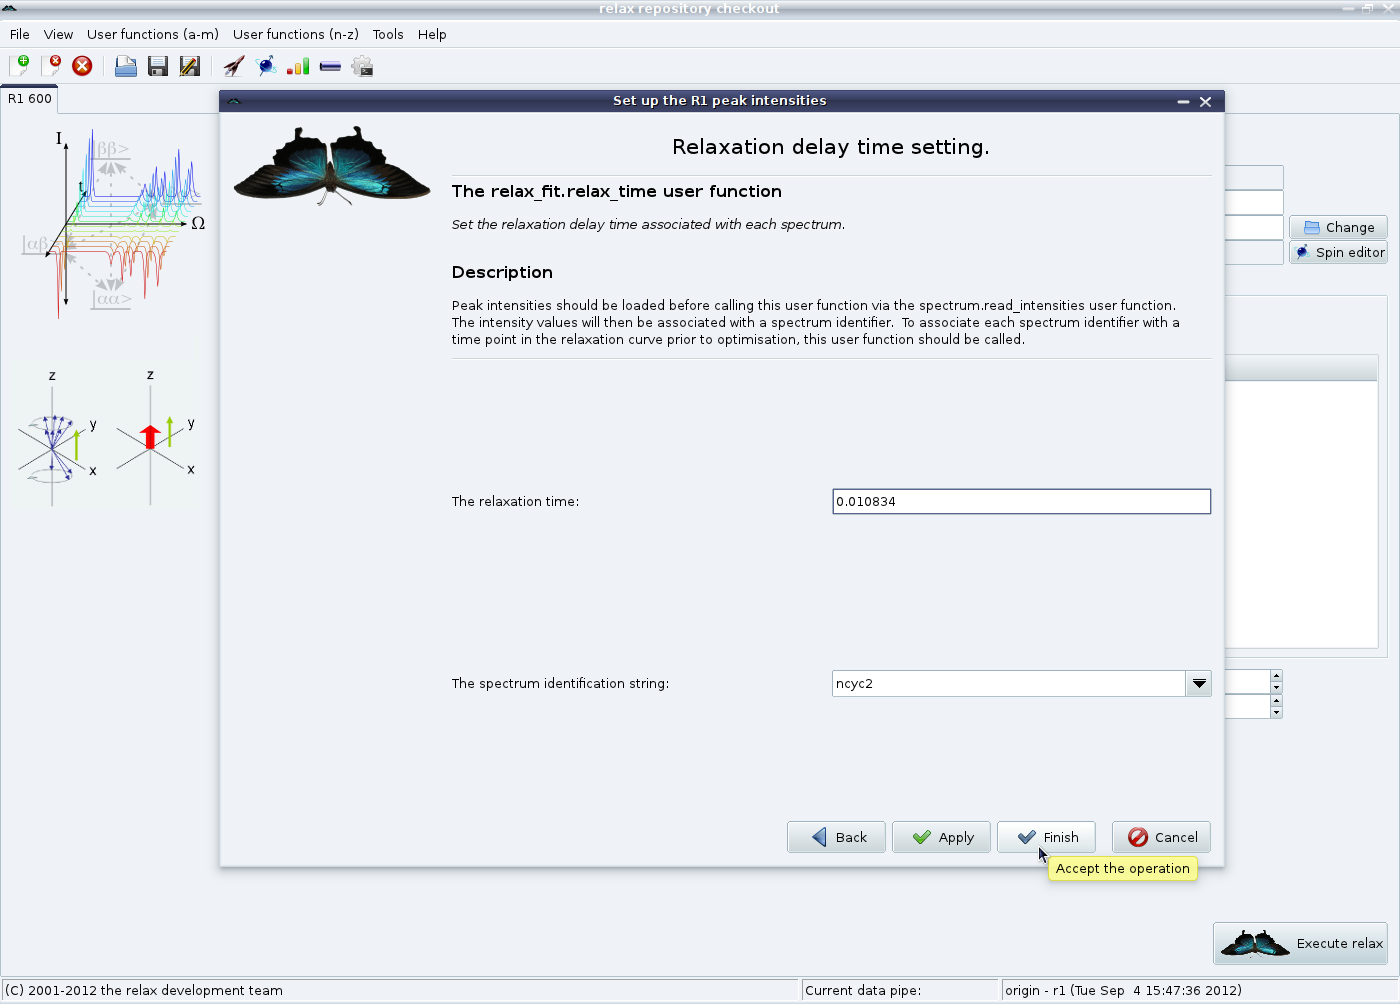
\includegraphics[
      width=0.8\textwidth,
      bb=14 14 1415 1019
    ]
    {graphics/screenshots/r1_analysis/peak_intensity_times}
  }
\end{minipage}

All delays and pulse lengths in the pulse sequence should be carefully checked to be sure that the time is exactly what you would expect -- the estimated time may not match the real time.
To set the time and close the wizard, click on the \guibutton{Finish} button.

This procedure should be repeated for every experiment you have collected (you could, as an alternative, load all at the same time using the \guibutton{Apply} button at each stage).
In the end you should see something such as:

\begin{minipage}[h]{\linewidth}
  \centerline{
    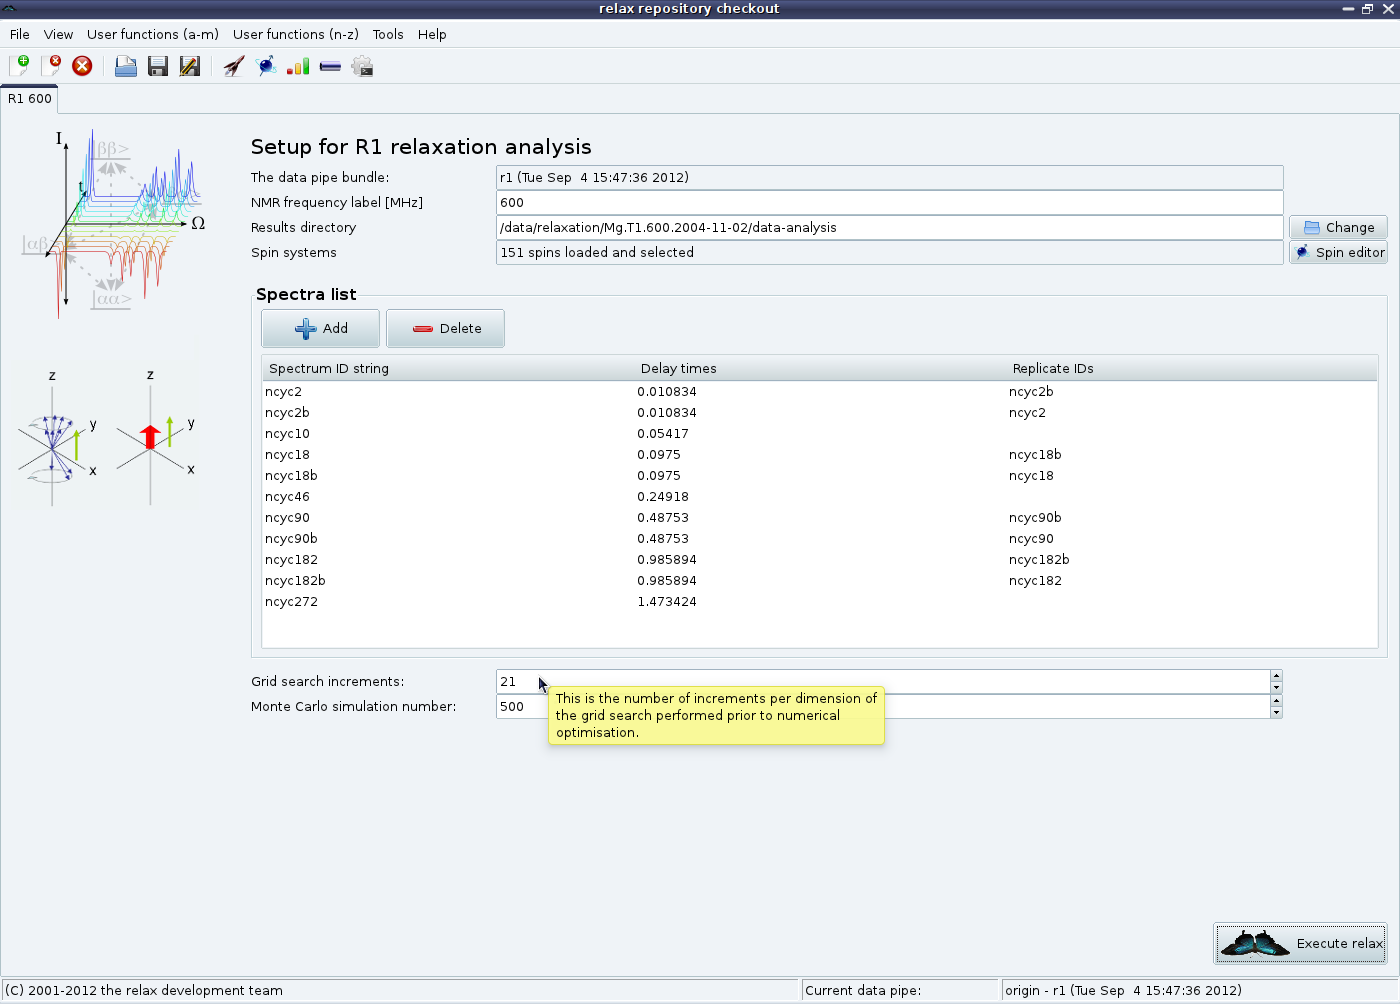
\includegraphics[
      width=0.8\textwidth,
      bb=14 14 1415 1019
    ]
    {graphics/screenshots/r1_analysis/analysis_tab_full}
  }
\end{minipage}


% Optimisation and error analysis.
%~~~~~~~~~~~~~~~~~~~~~~~~~~~~~~~~~

\subsection{Relax-fit GUI mode -- optimisation and error analysis}

Back in the main $\Rone$ analysis tab, the grid search increments and number of Monte Carlo simulations can be changed.
The default values of 21 grid search increments and 500 MC simulations are optimal -- lower values are not recommended.
To perform the optimisation and error analysis, click on the \guibutton{Execute relax} button.
The relax controller will open to show you the progress of the optimisation and simulations:

\begin{minipage}[h]{\linewidth}
  \centerline{
    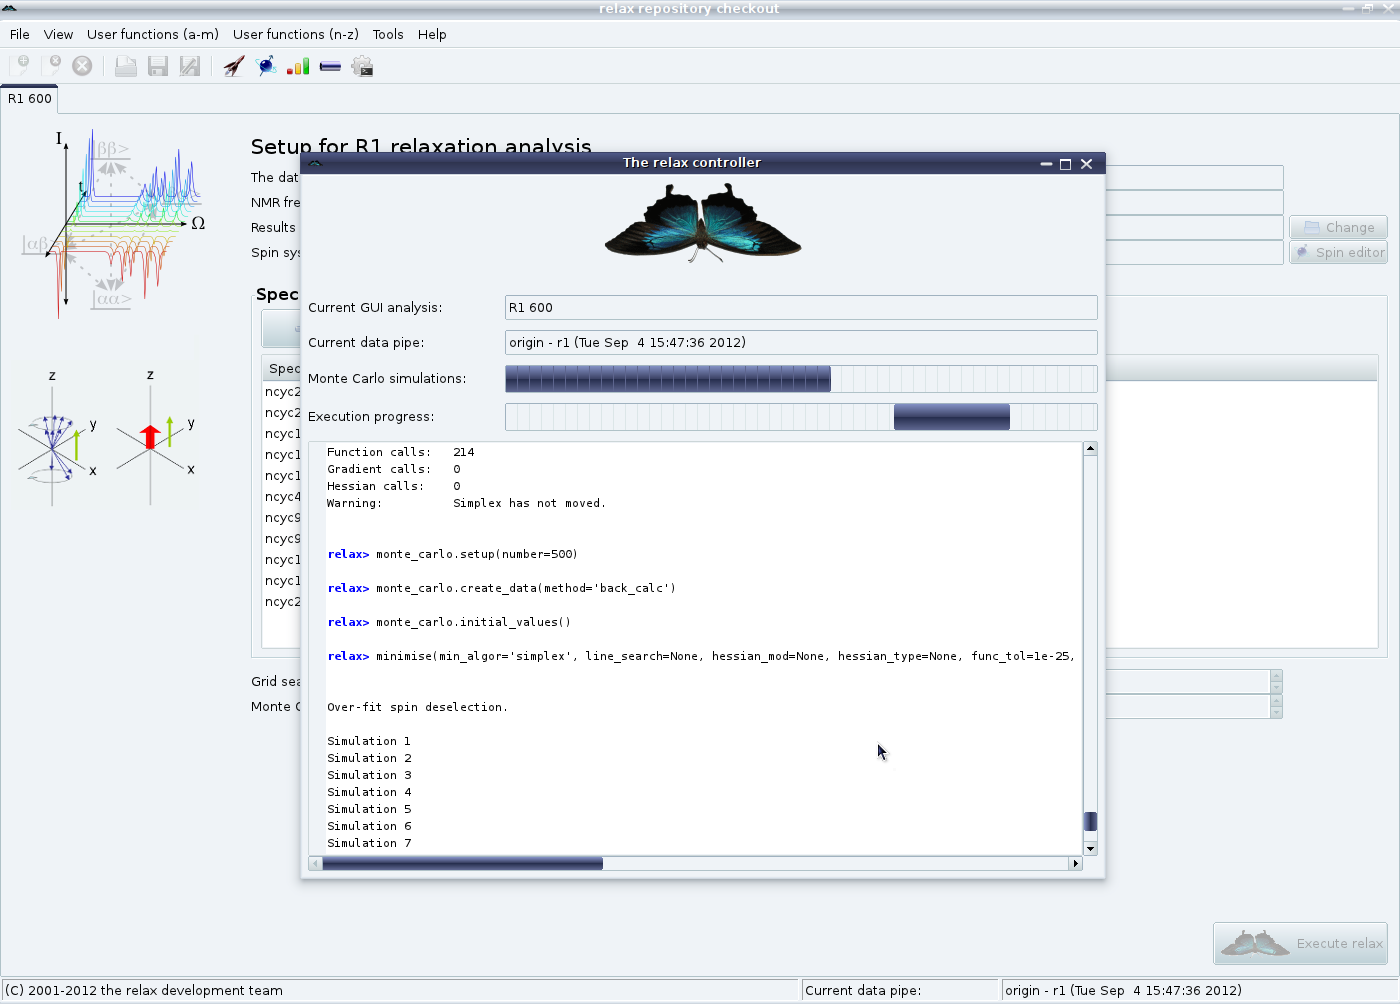
\includegraphics[
      width=0.8\textwidth,
      bb=14 14 1415 1019
    ]
    {graphics/screenshots/r1_analysis/mc_sim}
  }
\end{minipage}

Once finished, the \gui{Results viewer} window will also appear:

\begin{minipage}[h]{\linewidth}
  \centerline{
    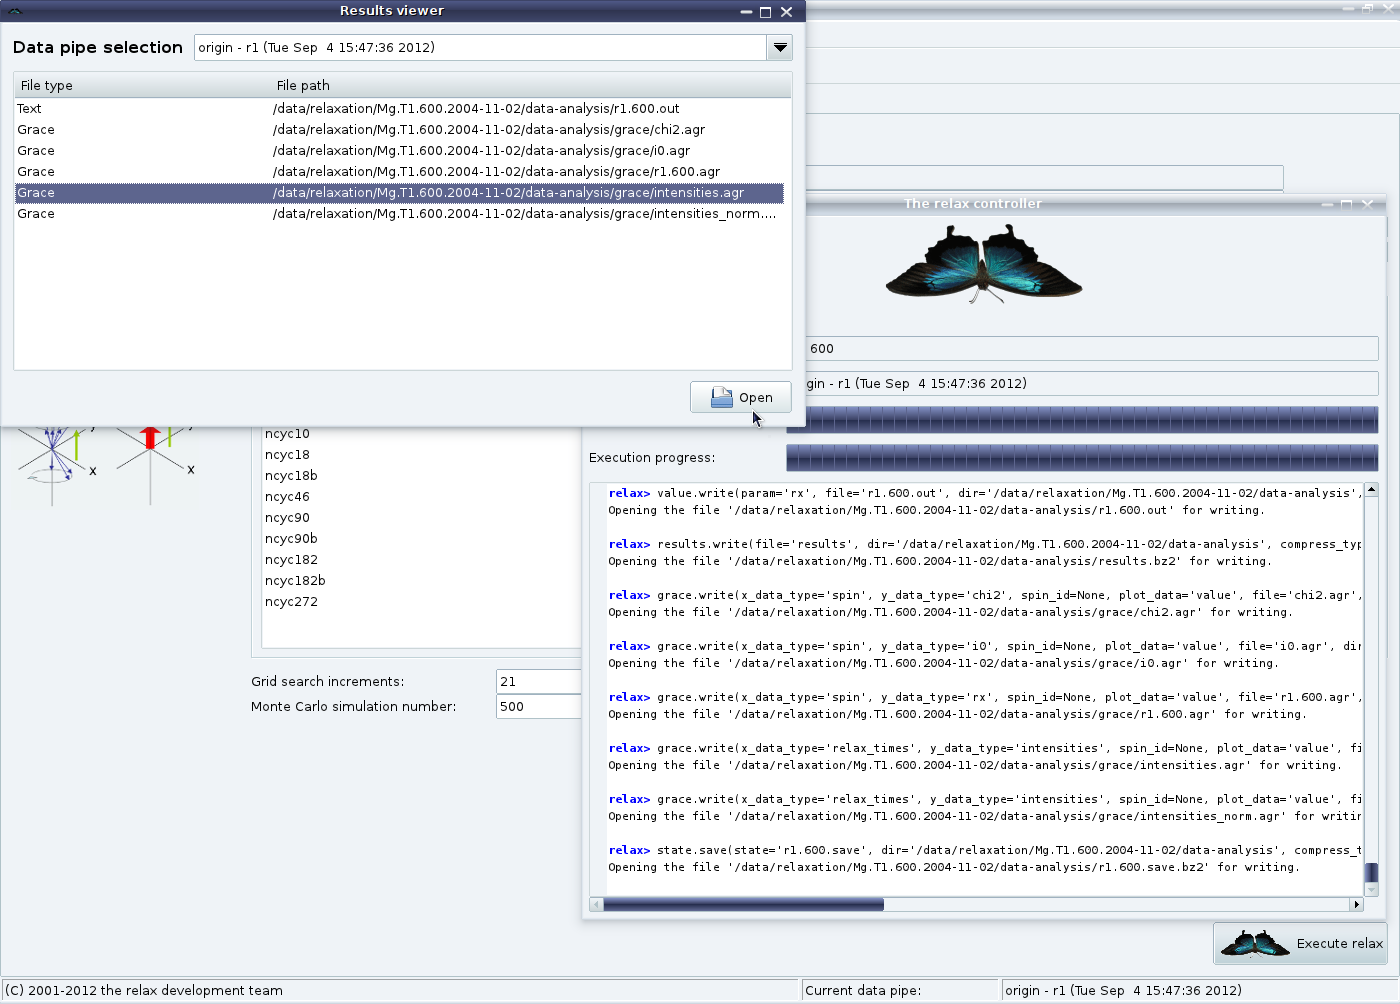
\includegraphics[
      width=0.8\textwidth,
      bb=14 14 1415 1019
    ]
    {graphics/screenshots/r1_analysis/fin}
  }
\end{minipage}

This window can be used to open the text files in the default text editor for your operating system or the 2D Grace plots in \prompt{xmgrace} if available on your system.



% Final checks.
%%%%%%%%%%%%%%%

\section{Final checks of the curve-fitting}

To be sure that the data has been properly collected and that no instrumentation or pulse sequence timing errors have occurred, it is essential to carefully check the \file{intensities.agr} and \file{intensities\osus{}norm.agr} 2D Grace\index{software!Grace|textbf} files.
These are plots of the decay curves for each spin system analysed, and any non-exponential behaviour should be clearly visible (see Figure~\ref{fig: screenshot: xmgrace peak intensities}).
If Xmgrace or a compatible program is not available for your operating system, the Grace files contain text representations of the curves at the end which can opened, edited and visualised in any another 2D graphing software package.
 
% Xmgrace screenshot
\begin{figure}
  \centerline{
    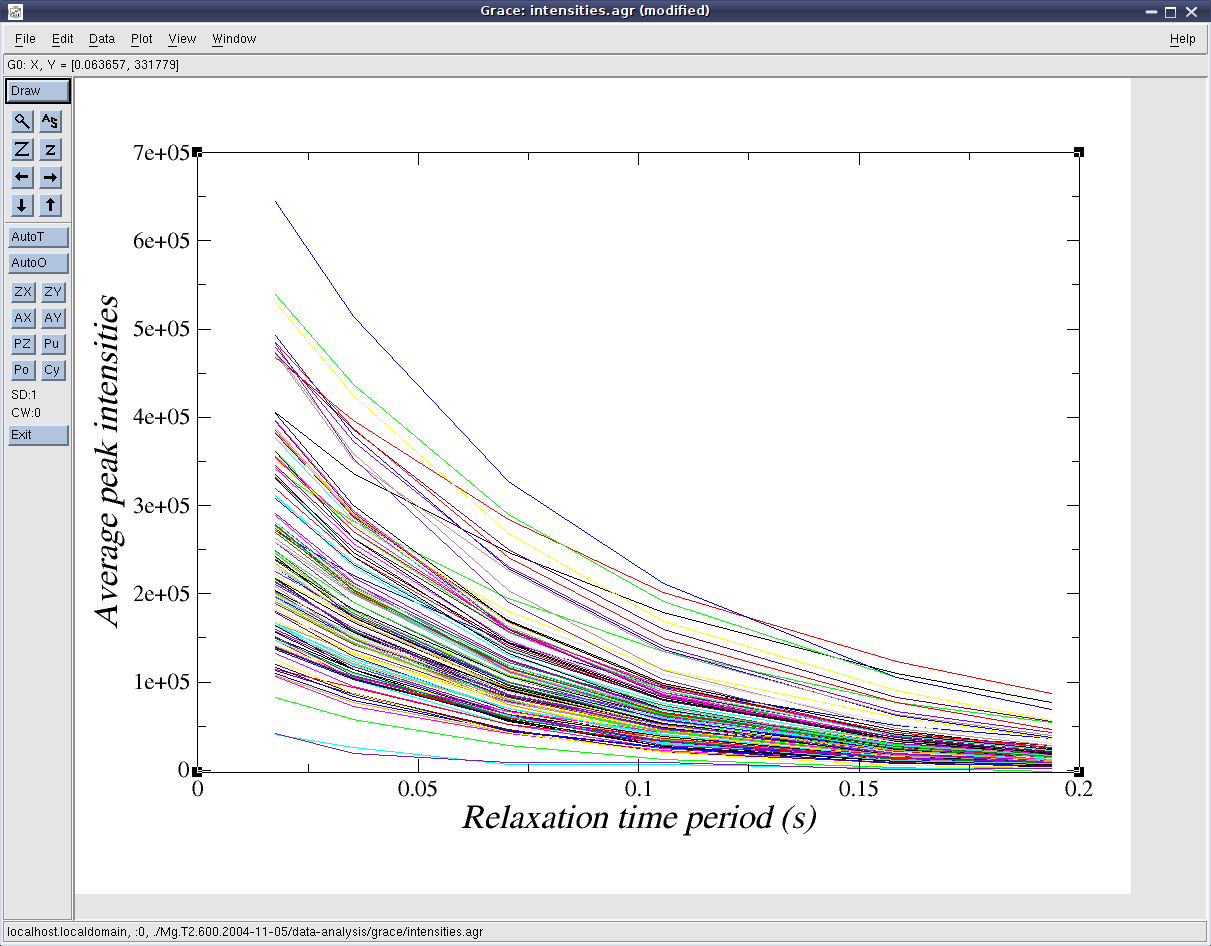
\includegraphics[
      width=\textwidth,
      bb=14 14 923 724
    ]
    {graphics/screenshots/xmgrace_peak_intensities}
  }
  \caption[Peak intensity 2D plot xmgrace screenshot]{
    Screenshot of the 2D peak intensity plots for the exponential relaxation curves in Xmgrace.
  }
  \label{fig: screenshot: xmgrace peak intensities}
\end{figure}

Note that errors resulting in systematic bias in the data -- for example if temperature control (single-scan interleaving or temperature compensation blocks) or per-experiment/per-spectrometer temperature calibration on MeOH or ethylene glycol have not been performed -- will not be detected by looking at the decay curves.
See section~\ref{sect: temperature control and calibration} or the \uf{relax\ufus{}data\ufsep{}temp\ufus{}calibration} user function documentation on page~\pageref{uf: relax_data.temp_calibration} and the \uf{relax\ufus{}data\ufsep{}temp\ufus{}control} user function documentation on page~\pageref{uf: relax_data.temp_control} for more details.
